% Figure 5: Learning Constraints Over Time — Diagnostic Plot
% Compile: pdflatex fig5_learning_curves.tex
%
% DATA REQUIRED:
%   Place these CSVs in the same directory (or adjust paths):
%     - constraint_violations.csv  (columns: epoch, jsc_negative, voc_negative,
%                                   vmpp_exceeds_voc, jmpp_exceeds_jsc, total_samples)
%     - multitask_losses.csv       (columns: epoch, sigma_anchor, sigma_curve)
%     - monotonicity.csv           (columns: epoch, region1_violations,
%                                   region2_violations, total_samples)
%
%   Generated by: python train.py --train-curves --device cuda
%   Output dir contains these files after training completes.
%
% If CSVs are not yet available, this file compiles with DEMO DATA (below).
% Comment out the demo \addplot sections and uncomment the \addplot table sections.

\documentclass[border=8pt]{standalone}
\usepackage{pgfplots}
\usepackage{amsmath}
\pgfplotsset{compat=1.18}
\usepgfplotslibrary{groupplots}

\definecolor{violred}{HTML}{C0392B}
\definecolor{monoteal}{HTML}{1ABC9C}
\definecolor{sigmagold}{HTML}{F39C12}
\definecolor{annotgray}{HTML}{7F8C8D}
\definecolor{gridlight}{HTML}{ECF0F1}

\begin{document}
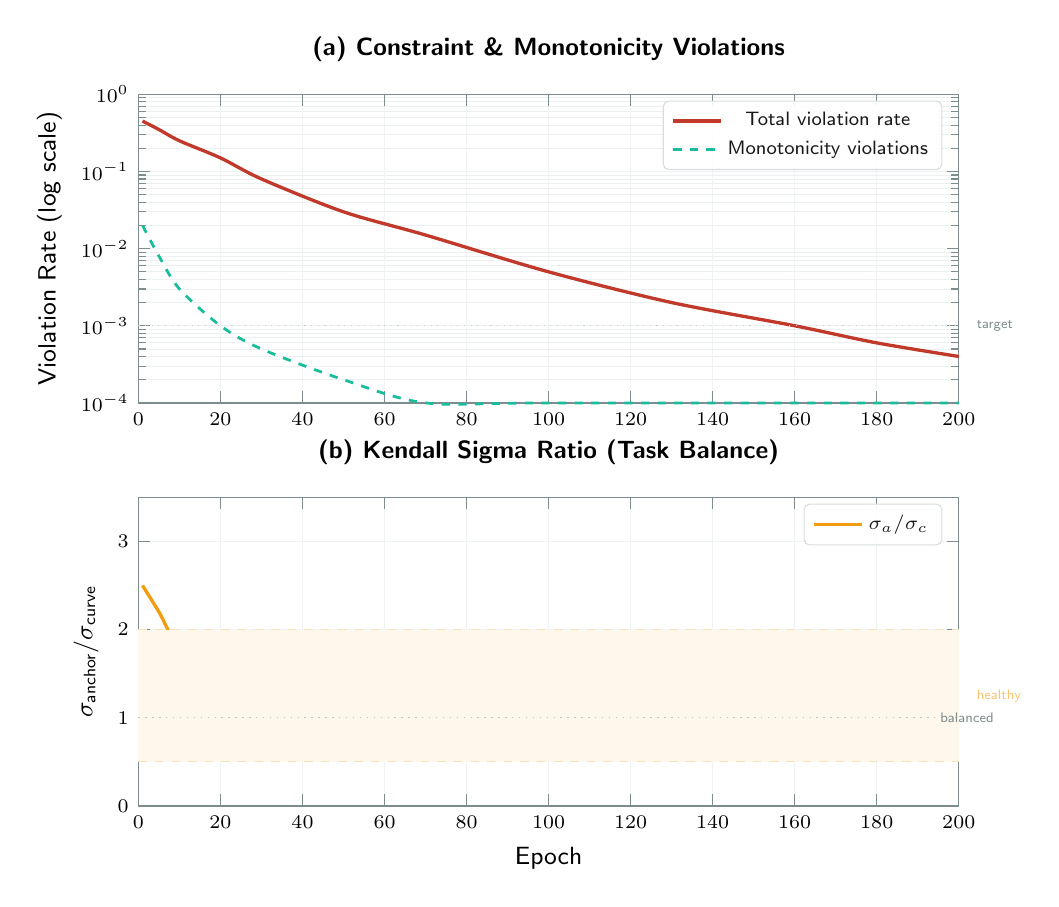
\begin{tikzpicture}

\begin{groupplot}[
  group style={
    group size=1 by 2,
    vertical sep=1.2cm,
    xlabels at=edge bottom,
  },
  width=12cm,
  height=5.5cm,
  xlabel={Epoch},
  xlabel style={font=\sffamily\small},
  ylabel style={font=\sffamily\small},
  tick label style={font=\sffamily\scriptsize},
  legend style={
    font=\sffamily\scriptsize,
    draw=annotgray!30,
    fill=white,
    fill opacity=0.9,
    rounded corners=2pt,
    at={(0.98,0.98)},
    anchor=north east,
  },
  grid=both,
  grid style={gridlight, line width=0.3pt},
  major grid style={gridlight!80, line width=0.4pt},
  axis line style={line width=0.5pt, annotgray},
  every tick/.style={annotgray},
  clip=false,
]

% ═══════════════════════════════════════════
% PANEL 1: Violation Rate + Monotonicity (log scale)
% ═══════════════════════════════════════════
\nextgroupplot[
  ylabel={Violation Rate (log scale)},
  ymode=log,
  ymin=1e-4, ymax=1,
  xmin=0, xmax=200,
  title={\sffamily\small\bfseries (a) Constraint \& Monotonicity Violations},
  title style={at={(0.5,1.02)}, anchor=south},
]

% ── DEMO DATA: Replace with CSV table reads ──
% Demo: exponential decay of violations over 200 epochs
\addplot[violred, line width=1.2pt, smooth, mark=none]
  coordinates {
    (1,0.45) (5,0.35) (10,0.25) (20,0.15) (30,0.08)
    (50,0.03) (70,0.015) (100,0.005) (130,0.002)
    (160,0.001) (180,0.0006) (200,0.0004)
  };
\addlegendentry{Total violation rate}

% Demo: monotonicity violations (should drop to ~0 quickly with cumsum)
\addplot[monoteal, line width=1.0pt, dashed, mark=none, smooth]
  coordinates {
    (1,0.02) (5,0.008) (10,0.003) (20,0.001) (30,0.0005)
    (50,0.0002) (70,0.0001) (100,0.0001) (200,0.0001)
  };
\addlegendentry{Monotonicity violations}

% ── TO USE REAL DATA, uncomment below and comment out demo plots above: ──
% \addplot[violred, line width=1.2pt, mark=none] table [
%   x=epoch,
%   y expr=(\thisrow{jsc_negative}+\thisrow{voc_negative}+\thisrow{vmpp_exceeds_voc}+\thisrow{jmpp_exceeds_jsc})/\thisrow{total_samples},
%   col sep=comma,
% ] {constraint_violations.csv};
% \addlegendentry{Total violation rate}
%
% \addplot[monoteal, line width=1.0pt, dashed, mark=none] table [
%   x=epoch,
%   y expr=(\thisrow{region1_violations}+\thisrow{region2_violations})/\thisrow{total_samples},
%   col sep=comma,
% ] {monotonicity.csv};
% \addlegendentry{Monotonicity violations}

% Annotation: target zero
\draw[annotgray!40, line width=0.4pt, dotted] (axis cs:0, 0.001) -- (axis cs:200, 0.001);
\node[font=\sffamily\tiny, text=annotgray, anchor=west] at (axis cs:202, 0.001) {target};

% ═══════════════════════════════════════════
% PANEL 2: Sigma Ratio (linear scale)
% ═══════════════════════════════════════════
\nextgroupplot[
  ylabel={$\sigma_{\text{anchor}} / \sigma_{\text{curve}}$},
  ymin=0, ymax=3.5,
  xmin=0, xmax=200,
  title={\sffamily\small\bfseries (b) Kendall Sigma Ratio (Task Balance)},
  title style={at={(0.5,1.02)}, anchor=south},
]

% Demo: sigma ratio starts erratic, stabilizes near 1.0
\addplot[sigmagold, line width=1.2pt, smooth, mark=none]
  coordinates {
    (1,2.5) (5,2.2) (10,1.8) (20,1.5) (30,1.3)
    (50,1.15) (70,1.08) (100,1.02) (130,0.98)
    (160,0.95) (180,0.93) (200,0.92)
  };
\addlegendentry{$\sigma_a / \sigma_c$}

% ── TO USE REAL DATA: ──
% \addplot[sigmagold, line width=1.2pt, mark=none] table [
%   x=epoch,
%   y expr=\thisrow{sigma_anchor}/\thisrow{sigma_curve},
%   col sep=comma,
% ] {multitask_losses.csv};
% \addlegendentry{$\sigma_a / \sigma_c$}

% Healthy band (0.1 to 10)
\fill[sigmagold!8] (axis cs:0, 0.5) rectangle (axis cs:200, 2.0);
\draw[sigmagold!30, line width=0.4pt, dashed] (axis cs:0, 0.5) -- (axis cs:200, 0.5);
\draw[sigmagold!30, line width=0.4pt, dashed] (axis cs:0, 2.0) -- (axis cs:200, 2.0);
\node[font=\sffamily\tiny, text=sigmagold!60, anchor=west] at (axis cs:202, 1.25) {healthy};

% Ideal ratio = 1 line
\draw[annotgray!50, line width=0.5pt, dotted] (axis cs:0, 1.0) -- (axis cs:200, 1.0);
\node[font=\sffamily\tiny, text=annotgray] at (axis cs:202, 1.0) {balanced};

\end{groupplot}

\end{tikzpicture}
\end{document}
